\chapter{Réalisation et Implémentation}
\label{chap:implementation}


\section{Introduction}
\label{sec:introduction_implementation}

Après avoir présenté l’analyse et la conception de notre système, ce chapitre est consacré à la réalisation pratique de l’application. Il permet de montrer comment les besoins définis précédemment ont été transformés en une solution web fonctionnelle pour la gestion du courrier.

Dans cette partie, nous présentons d’abord les outils et technologies utilisés durant le développement, notamment Laravel pour la partie serveur, React pour l’interface utilisateur, ainsi que les autres bibliothèques et services nécessaires au bon fonctionnement de l’application. Ensuite, nous expliquons le principe de communication entre le front-end et le back-end à travers une API REST, avant de donner un aperçu des principales interfaces réalisées.

Ce chapitre permet donc de passer de la conception théorique à l’implémentation réelle du système, en mettant en évidence les choix techniques adoptés et leur rôle dans le fonctionnement global de l’application.
\section{Environnement et outils de développement}
Le développement de notre application repose sur plusieurs outils utilisés pour gérer le serveur, l’interface, la base de données, la communication et la conception du système.

\subsection{Laravel}
\label{subsec:laravel}

\begin{figure}[H]
    \centering
    % Image à ajouter : logo officiel de Laravel
    % Exemple : images/laravel_logo.png
    
\includegraphics[width=0.25\textwidth]{images/logos/laravel.png}
    \caption{Logo du framework Laravel}
    \label{fig:laravel_logo}
\end{figure}

Laravel est un framework PHP utilisé dans notre projet pour gérer la logique de l’application, les routes, les contrôleurs, les modèles et les échanges avec la base de données. D’après la documentation officielle, Laravel est présenté comme un framework destiné au développement d’applications web en PHP \cite{laravel}. Il ne se limite pas seulement à l’écriture du code serveur, car il propose aussi plusieurs outils autour du développement, comme l’authentification, les notifications, les files d’attente, les migrations, Eloquent ORM, Sanctum et Reverb \cite{laraveldocs}. C’est pour cette raison que Laravel peut être considéré comme un écosystème complet. Dans notre application, il nous a surtout permis de créer une API RESTful, utilisée par l’interface React pour envoyer des requêtes, récupérer les données et effectuer les différentes opérations liées à la gestion du courrier.
\subsubsection{Eloquent ORM}
\label{subsubsec:eloquent_orm}

Eloquent ORM est l’outil de Laravel qui permet de travailler avec la base de données d’une manière plus simple. Au lieu d’écrire directement des requêtes SQL dans tout le projet, on utilise des classes appelées \textit{models}. Chaque modèle représente généralement une table de la base de données. Par exemple, dans notre application, un modèle \texttt{Courrier} peut représenter la table des courriers, tandis qu’un modèle \texttt{User} représente les utilisateurs du système. D’après la documentation officielle de Laravel, Eloquent associe chaque table de la base à un modèle qui permet de récupérer, ajouter, modifier ou supprimer les enregistrements \cite{laravel_eloquent}.

Dans notre projet, Eloquent nous a aidés à organiser la partie liée aux données. Les courriers, les utilisateurs, les pièces jointes, les commentaires et les messages peuvent être manipulés à partir de modèles. Cela rend le code plus lisible, surtout lorsque plusieurs opérations doivent être faites sur les mêmes données. Par exemple, au lieu d’écrire une requête SQL pour chercher les courriers reçus, on peut utiliser une méthode du modèle \texttt{Courrier}.

\begin{lstlisting}[language=PHP, caption={Exemple simple de modèle Eloquent}]
class Courrier extends Model
{
    protected $fillable = [
        'objet',
        'type',
        'statut',
        'priorite',
        'user_id',
        'structure_id'
    ];
}
\end{lstlisting}

Un autre point important dans Eloquent est la gestion des relations entre les tables. Dans une application de gestion de courrier, un courrier peut appartenir à un utilisateur, avoir plusieurs pièces jointes ou recevoir plusieurs commentaires. Ces relations peuvent être écrites directement dans les modèles. La documentation Laravel précise que les relations Eloquent sont définies comme des méthodes dans les classes des modèles, ce qui permet ensuite de les utiliser facilement dans les requêtes \cite{laravel_relationships}.

\begin{lstlisting}[language=PHP, caption={Exemple de relations dans un modèle Courrier}]
class Courrier extends Model
{
    public function utilisateur()
    {
        return $this->belongsTo(User::class, 'user_id');
    }

    public function piecesJointes()
    {
        return $this->hasMany(CourrierAttachment::class);
    }

    public function commentaires()
    {
        return $this->hasMany(CourrierComment::class);
    }
}
\end{lstlisting}

Les \textit{scopes} sont aussi très utiles dans Eloquent. Ils permettent de regrouper des conditions de recherche que l’on utilise souvent. Par exemple, dans notre application, on peut avoir besoin d’afficher seulement les courriers reçus, les courriers archivés ou les courriers en attente de validation. Au lieu de répéter les mêmes conditions dans plusieurs contrôleurs, on peut les mettre une seule fois dans le modèle. Laravel distingue notamment les scopes locaux et les scopes globaux. Les scopes locaux servent à réutiliser une condition précise dans certaines requêtes, alors que les scopes globaux s’appliquent automatiquement à toutes les requêtes d’un modèle \cite{laravel_eloquent}.

\begin{lstlisting}[language=PHP, caption={Exemple de scopes locaux pour les courriers}]
class Courrier extends Model
{
    public function scopeRecus($query)
    {
        return $query->where('type', 'recu');
    }

    public function scopeArchives($query)
    {
        return $query->where('statut', 'archive');
    }

    public function scopeEnAttente($query)
    {
        return $query->where('statut', 'en_attente');
    }
}
\end{lstlisting}

Après la définition de ces scopes, leur utilisation devient plus claire dans le contrôleur :

\begin{lstlisting}[language=PHP, caption={Utilisation des scopes dans un contrôleur}]
$courriersRecus = Courrier::recus()->get();

$courriersArchives = Courrier::archives()
    ->where('structure_id', $structureId)
    ->get();

$courriersEnAttente = Courrier::enAttente()->get();
\end{lstlisting}

Eloquent propose aussi d’autres fonctionnalités pratiques, comme les migrations, les timestamps automatiques, la suppression douce avec \texttt{SoftDeletes}, ainsi que les \textit{casts}. Les casts permettent de transformer automatiquement certains champs lorsqu’ils sont lus ou enregistrés. Par exemple, un champ de type date peut être manipulé directement comme un objet date, et un champ JSON peut être converti automatiquement en tableau PHP. La documentation officielle indique que les accessors, mutators et casts permettent de transformer les valeurs des attributs lorsqu’elles sont récupérées ou définies dans un modèle \cite{laravel_mutators}.

Dans notre application, Eloquent a donc joué un rôle important dans la communication avec la base de données. Il a permis de garder un code plus propre, de limiter la répétition des requêtes et de mieux représenter les éléments principaux du système sous forme de modèles liés entre eux.

\subsubsection{Laravel Sanctum}
\label{subsubsec:sanctum}
Laravel Sanctum est un package officiel de Laravel consacré à l’authentification. Il permet de sécuriser les applications de type SPA, les applications mobiles ainsi que les API simples basées sur des tokens \cite{laravel_sanctum}. Son rôle est de vérifier l’identité de l’utilisateur avant de lui donner accès aux ressources protégées. Il peut fonctionner soit avec les cookies de session, soit avec des tokens d’API envoyés avec les requêtes. Sanctum reste donc une solution assez simple à mettre en place, sans passer par un système plus lourd comme OAuth.

\subsubsection{Laravel Reverb}
\label{subsubsec:reverb}

\begin{figure}[H]
    \centering
    % Image à ajouter : logo officiel de Laravel Reverb
    % Exemple : images/reverb_logo.png
    
\includegraphics[width=0.25\textwidth]{images/logos/reverb_logo.png}
    \caption{Logo de Laravel Reverb}
    \label{fig:reverb_logo}
\end{figure}

Laravel Reverb est le serveur WebSocket officiel de Laravel. Il permet d’ajouter des échanges en temps réel dans une application, comme les notifications ou les messages instantanés. Reverb fonctionne avec le broadcasting de Laravel et reste compatible avec Laravel Echo grâce au protocole Pusher \cite{laravel_reverb}.
\subsection{React}
\label{subsec:react}

\begin{figure}[H]
    \centering
    % Image à ajouter : logo officiel de React
    % Exemple : images/react_logo.png
    
\includegraphics[width=0.22\textwidth]{images/logos/react_logo.png}
    \caption{Logo de React}
    \label{fig:react_logo}
\end{figure}

React est une bibliothèque JavaScript utilisée pour créer des interfaces utilisateur. Le site officiel la présente comme \textit{``the library for web and native user interfaces''} \cite{react}. Dans notre projet, React est utilisé pour construire les pages et les composants visibles par l’utilisateur.

\subsubsection{React Router DOM}
\label{subsubsec:react_router_dom}

React Router DOM permet de gérer la navigation entre les pages d’une application React. Il relie les URL aux composants affichés, ce qui permet de passer d’une page à une autre sans recharger toute l’application \cite{react_router}.

\subsubsection{Axios}
\label{subsubsec:axios}

\begin{figure}[H]
    \centering
    % Image à ajouter : logo officiel d'Axios
    % Exemple : images/axios_logo.png
    
\includegraphics[width=0.22\textwidth]{images/logos/axios_logo.png}
    \caption{Logo d’Axios}
    \label{fig:axios_logo}
\end{figure}

Axios est un client HTTP utilisé pour envoyer des requêtes vers une API. Sa documentation le définit comme un client HTTP simple pour le navigateur et Node.js \cite{axios}. Dans notre application, il sert surtout à envoyer les requêtes depuis React vers le serveur Laravel.
\subsection{Tailwind CSS}
\label{subsec:tailwind}
\begin{figure}[H]
    \centering
    % Image à ajouter : logo officiel de Tailwind CSS
    % Exemple : images/tailwind_logo.png
    
\includegraphics[width=0.22\textwidth]{images/logos/tailwind_logo.png}
    \caption{Logo de Tailwind CSS}
    \label{fig:tailwind_logo}
\end{figure}
Tailwind CSS est \textit{``a utility-first CSS framework for rapidly building modern websites without ever leaving your HTML''} \cite{tailwind}. Dans notre application, il sert surtout à styliser les composants React et à rendre l’interface plus claire, moderne et responsive.

\subsection{PlantUML}
\label{subsec:plantuml}

\begin{figure}[H]
    \centering
    % Image à ajouter : logo PlantUML
    % Exemple : images/plantuml_logo.png
    
\includegraphics[width=0.22\textwidth]{images/logos/plantuml_logo.png}
    \caption{Logo de PlantUML}
    \label{fig:plantuml_logo}
\end{figure}

PlantUML est un composant qui permet de dessiner rapidement des diagrammes UML à l’aide d’un langage simple et intuitif \cite{plantuml}.
\subsection{XAMPP}
\label{subsec:xampp}

\begin{figure}[H]
    \centering
    % Image à ajouter : logo XAMPP
    
\includegraphics[width=0.20\textwidth]{images/logos/xampp_logo.png}
    \caption{Logo de XAMPP}
    \label{fig:xampp_logo}
\end{figure}

XAMPP est une distribution Apache facile à installer qui contient MariaDB, PHP et Perl \cite{xampp}.

\subsubsection{MariaDB / MySQL}
\label{subsubsec:mariadb_mysql}

\begin{figure}[H]
    \centering
    % Image à ajouter : logo MariaDB
    
\includegraphics[width=0.22\textwidth]{images/logos/mariadb_logo.png}
    \caption{Logo de MariaDB}
    \label{fig:mariadb_logo}
\end{figure}

MariaDB Server est un système de gestion de base de données relationnelle open source \cite{mariadb}.

\subsubsection{Apache Server}
\label{subsubsec:apache_server}

\begin{figure}[H]
    \centering
    % Image à ajouter : logo Apache
    
\includegraphics[width=0.22\textwidth]{images/logos/apache_logo.png}
    \caption{Logo d'Apache HTTP Server}
    \label{fig:apache_logo}
\end{figure}

Apache HTTP Server est un serveur HTTP open source pour les systèmes d’exploitation modernes, y compris UNIX et Windows \cite{apache}.

\subsection{OCR}
\label{subsec:ocr}

\begin{figure}[H]
    \centering
    % Image à ajouter : logo Tesseract OCR
    
\includegraphics[width=0.22\textwidth]{images/logos/tesseract_logo.png}
    \caption{Logo de Tesseract OCR}
    \label{fig:tesseract_logo}
\end{figure}

Tesseract est un moteur de reconnaissance de texte open source OCR, disponible sous licence Apache 2.0 \cite{tesseract}. Dans notre projet, nous avons utilisé \texttt{tesseract.exe} pour extraire le texte à partir des documents numérisés.

\section{API RESTful}
\label{sec:api_restful}

Une API REST est une interface de programmation d'application qui respecte les principes de conception du style d'architecture REST \cite{rest_api}.

\section{Cycle de traitement d’une requête Laravel}
\label{sec:cycle_requete_laravel}

Dans une application Laravel, le traitement commence lorsqu’une requête HTTP arrive vers l’application. Le fichier \texttt{index.php} est le point d’entrée de toutes les requêtes, puis Laravel charge l’application et transmet la requête vers le routeur \cite{laravel_lifecycle}. Dans notre projet, cette requête peut être envoyée depuis React avec Axios. Axios est un \textit{``Promise based HTTP client for the browser and node.js''} \cite{axios}. Il permet donc d’envoyer une demande vers un endpoint Laravel, par exemple pour récupérer la liste des courriers ou enregistrer un nouveau courrier.

\begin{figure}[H]
    \centering
    % Image à ajouter : schéma du cycle d’une requête Laravel
    % Exemple : images/laravel_request_cycle.png
    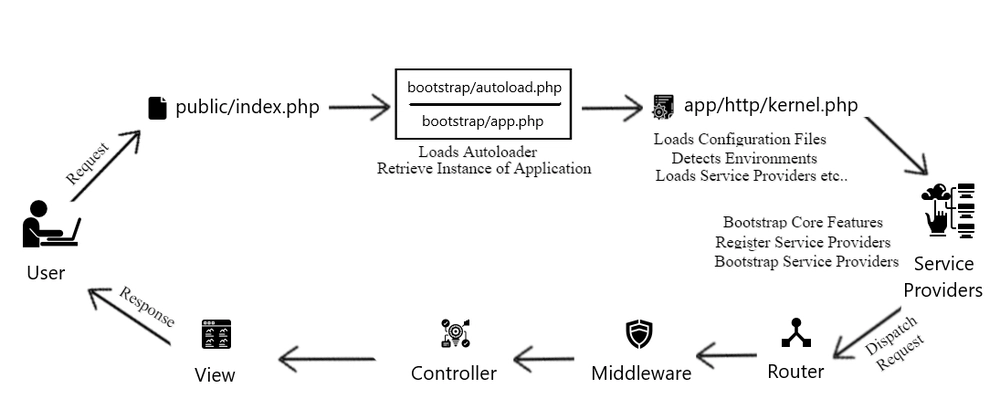
\includegraphics[width=0.85\textwidth]{images/logos/laravel_request_cycle.png }
    \caption{Cycle de traitement d’une requête Laravel\cite{patel_laravel_lifecycle}}
    \label{fig:laravel_request_cycle}
\end{figure}

Après l’arrivée de la requête, Laravel cherche la route correspondante, applique les middlewares nécessaires, puis exécute le contrôleur associé. La validation peut intervenir avant le traitement pour vérifier les données envoyées par l’utilisateur. Ensuite, le contrôleur utilise souvent un modèle Eloquent pour lire ou modifier les données dans la base. Une fois le traitement terminé, la réponse revient vers le client. Laravel précise que \textit{``All routes and controllers should return a response to be sent back to the user's browser''} \cite{laravel_responses}. Dans le cas d’une API, cette réponse est souvent envoyée au format JSON. JSON est un format textuel utilisé pour représenter des données structurées, ce qui le rend pratique pour transmettre les résultats vers le front-end \cite{mdn_json}. L’interface React peut ensuite exploiter ces données pour afficher les informations à l’utilisateur.
\section{Aperçu de l'application réalisée}
\label{sec:apercu_application}

Cette section présente ce qu’on voit dans l’application après avoir développé les pages principales. L’idée est de donner une première image de l’interface et des fonctionnalités, sans entrer dans le code.

\subsection{Tableau de bord}
\label{subsec:dashboard}

Le tableau de bord est la page d’accueil après connexion. On y trouve un résumé rapide des courriers et des notifications, pour savoir tout de suite si quelque chose demande une action.

\begin{figure}[H]
    \centering
    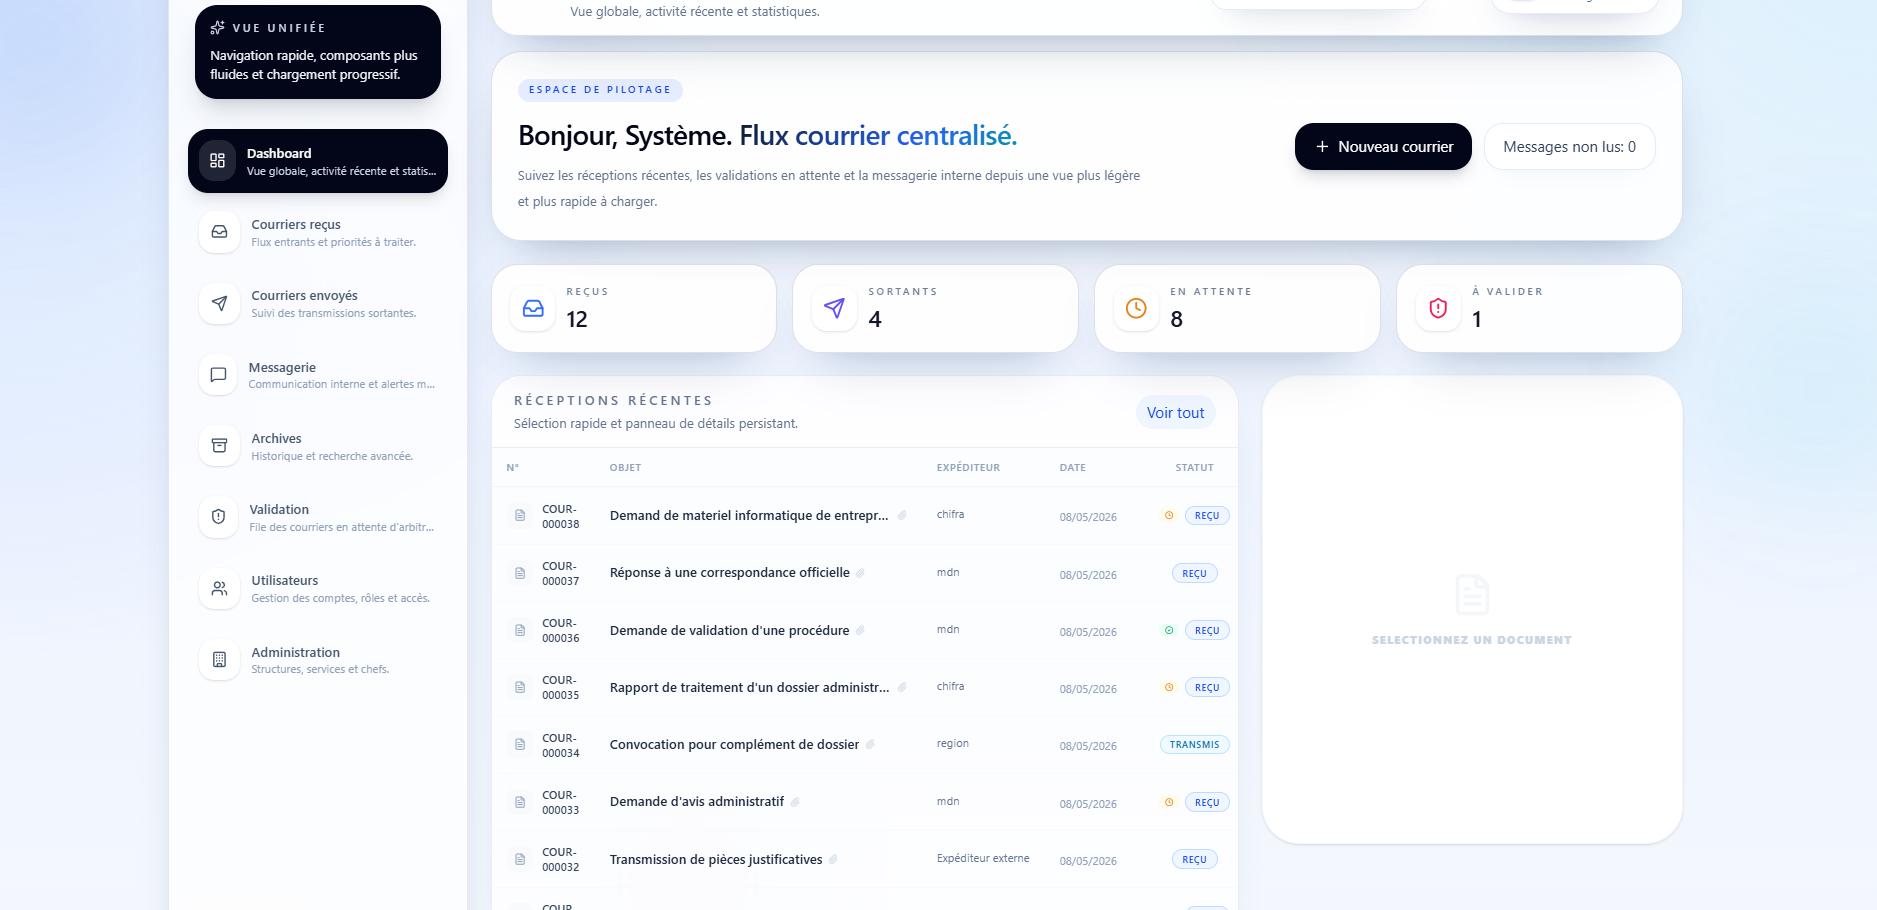
\includegraphics[width=0.92\textwidth,height=0.46\textheight,keepaspectratio]{images/app/dashboard.png}
    \caption{Vue du tableau de bord}
    \label{fig:dashboard_preview}
\end{figure}

\subsection{Gestion des courriers reçus}
\label{subsec:courriers_recus}

Cette partie du site regroupe tous les courriers entrants traités par l’application. L’utilisateur peut consulter la liste, filtrer et aller vers un courrier précis.

\begin{figure}[H]
    \centering
    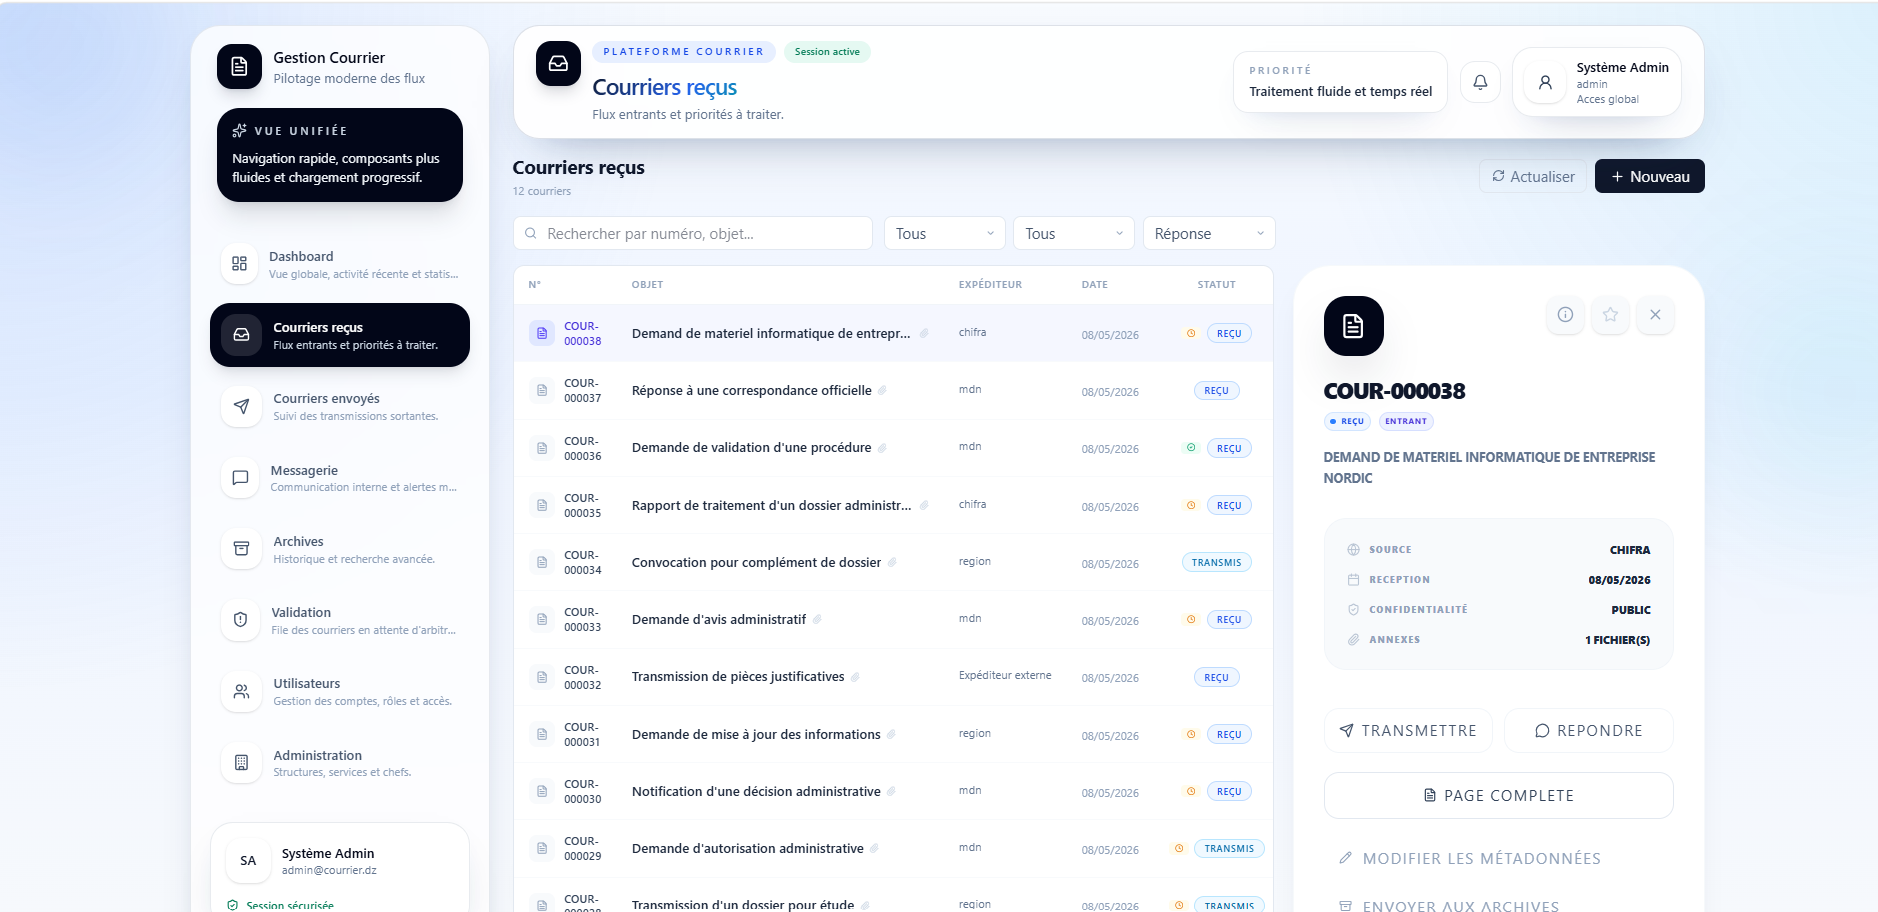
\includegraphics[width=0.92\textwidth,height=0.46\textheight,keepaspectratio]{images/app/courier_recu.png}
    \caption{Liste des courriers reçus}
    \label{fig:courriers_recus_list}
\end{figure}

\subsubsection{Création d’un nouveau courrier reçu}
\label{subsubsec:creation_courrier_recu}

La création d’un courrier reçu se fait avec un formulaire qui accepte l’objet, le service destinataire, la date et les pièces jointes. C’est la base pour entrer les documents qui arrivent dans l’organisation.

\begin{figure}[H]
    \centering
    \begin{minipage}{0.49\textwidth}
        \centering
        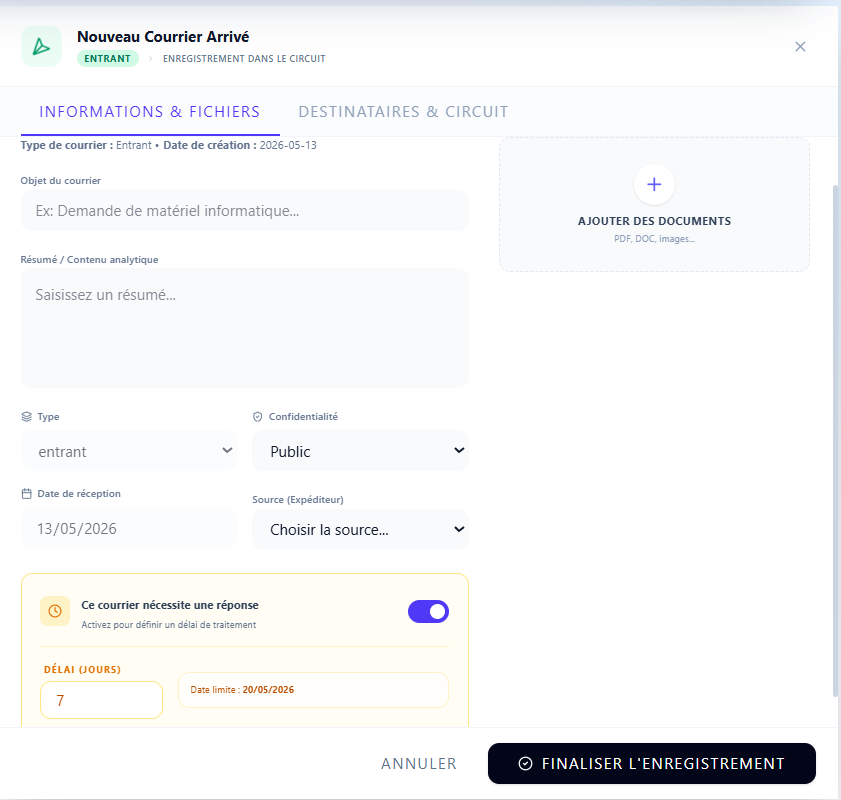
\includegraphics[width=\linewidth,height=0.36\textheight,keepaspectratio]{images/app/courier_recu_crre1.png}
    \end{minipage}
    \hfill
    \begin{minipage}{0.49\textwidth}
        \centering
        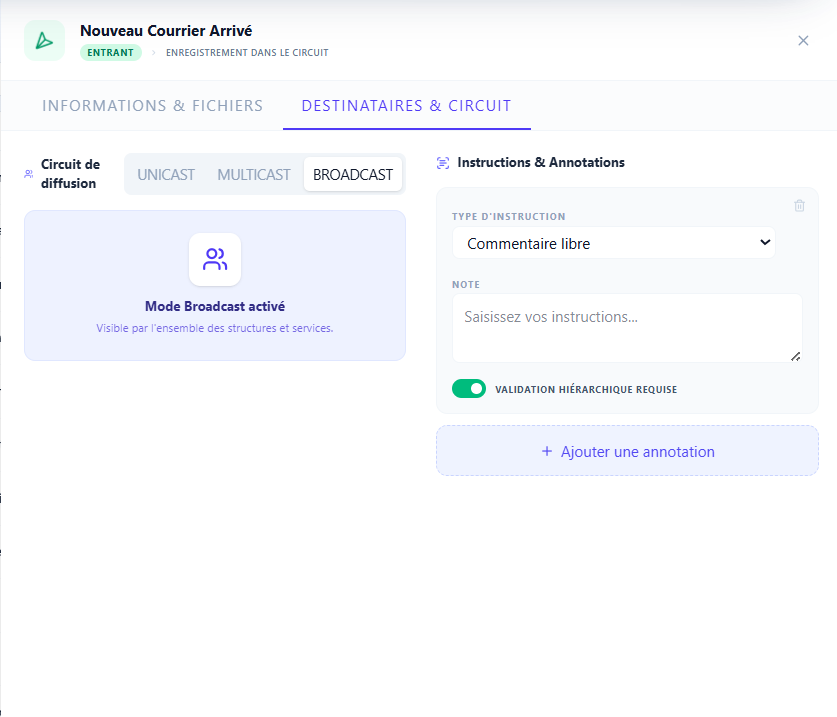
\includegraphics[width=\linewidth,height=0.36\textheight,keepaspectratio]{images/app/courier_recu_crr2.png}
    \end{minipage}
    \caption{Formulaire de création d’un courrier reçu}
    \label{fig:creation_courrier_recu}
\end{figure}

\subsubsection{Transmission d’un courrier}
\label{subsubsec:transmission_courrier}

Quand il faut transférer un courrier vers un autre service ou responsable, la transmission permet d’avancer le dossier. L’interface propose un bouton de transmission et un suivi d’état simple.

\begin{figure}[H]
    \centering
    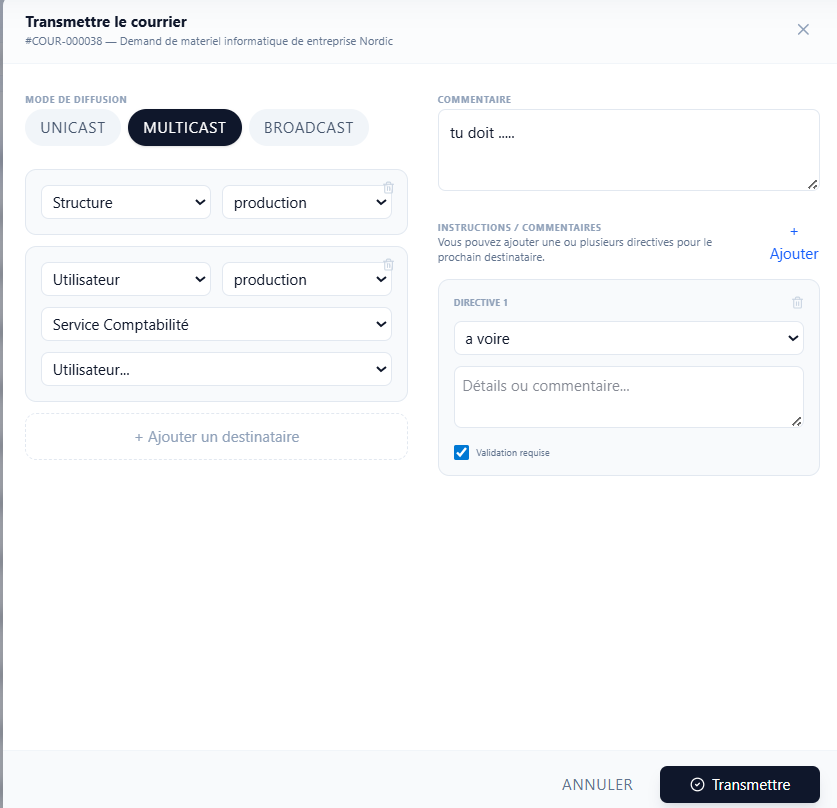
\includegraphics[width=0.90\textwidth,height=0.44\textheight,keepaspectratio]{images/app/trans.png}
    \caption{Écran de transmission d’un courrier}
    \label{fig:transmission_courrier}
\end{figure}

\subsubsection{Réponse à un courrier}
\label{subsubsec:reponse_courrier}

La réponse à un courrier s’effectue depuis le détail du courrier reçu, avec un formulaire pré-rempli et des destinataires suggérés selon le workflow.

\begin{figure}[H]
    \centering
    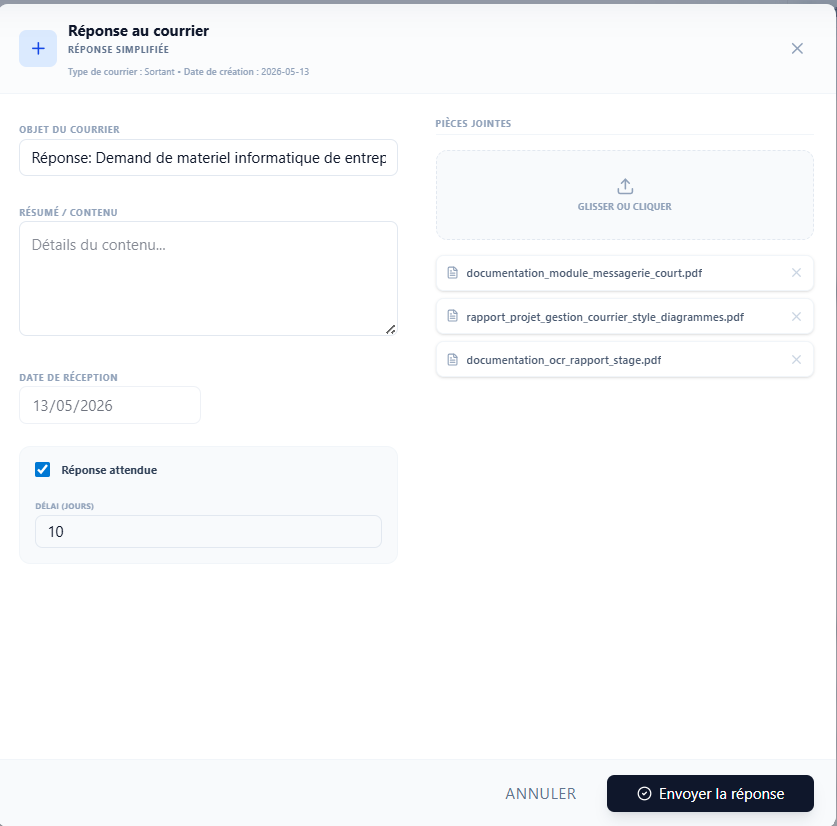
\includegraphics[width=0.90\textwidth,height=0.3\textheight,keepaspectratio]{images/app/respo_cor.png}
    \caption{Interface de réponse à un courrier}
    \label{fig:reponse_courrier}
\end{figure}

\subsubsection{Archivage d’un courrier}
\label{subsubsec:archivage_courrier}

L’archivage permet de ranger un courrier hors du flux actif, tout en le gardant accessible pour consultation future. Le système retire le courrier de la vue principale sans le supprimer.

\begin{figure}[H]
    \centering
    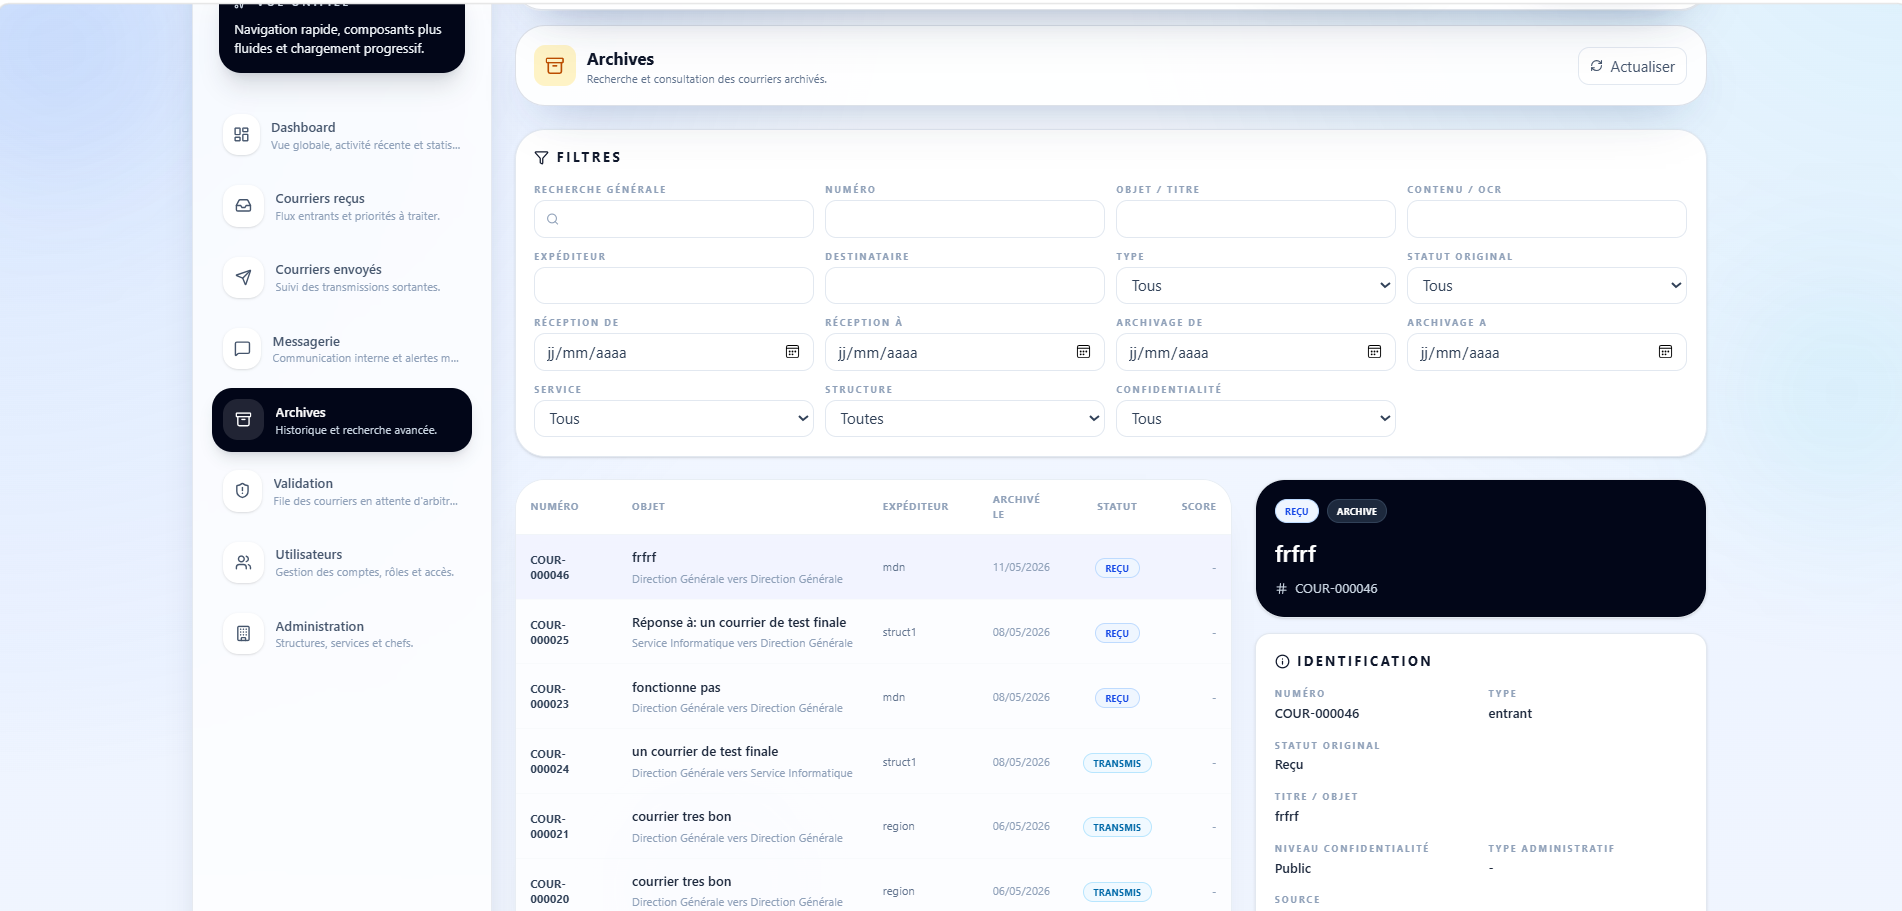
\includegraphics[width=0.90\textwidth,height=0.44\textheight,keepaspectratio]{images/app/archive.png}
    \caption{Archivage d’un courrier}
    \label{fig:archivage_courrier}
\end{figure}


\subsection{Gestion des courriers envoyés}
\label{subsec:courriers_envoyes}

Cette section liste les courriers sortants. Elle montre les envois déjà effectués, les brouillons et les éléments en attente de validation.

\begin{figure}[H]
    \centering
    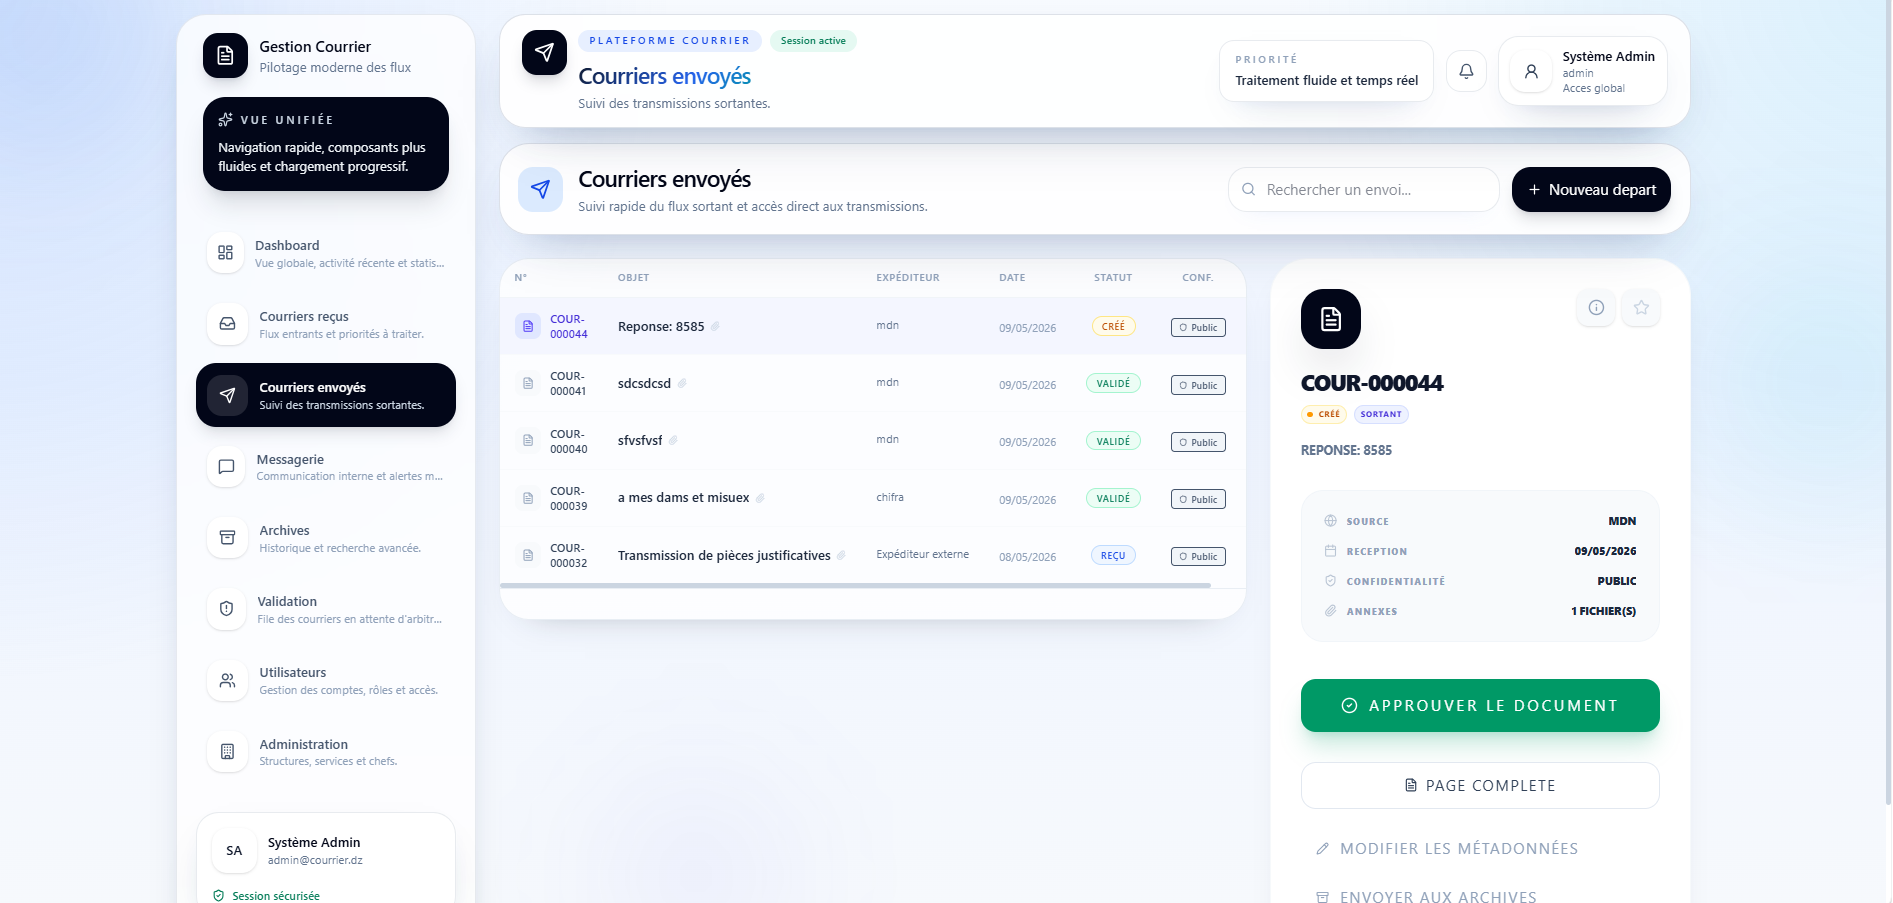
\includegraphics[width=0.92\textwidth,height=0.40\textheight,keepaspectratio]{images/app/courrier_env.png}
    \caption{Liste des courriers envoyés}
    \label{fig:courriers_envoyes}
\end{figure}

\subsubsection{Création d’un nouveau courrier envoyé}
\label{subsubsec:creation_courrier_envoye}

Le formulaire d’envoi permet de rédiger un courrier sortant, de choisir la confidentialité et les destinataires, puis de l’enregistrer ou de le soumettre.

\begin{figure}[H]
    \centering
    \begin{minipage}{0.49\textwidth}
        \centering
        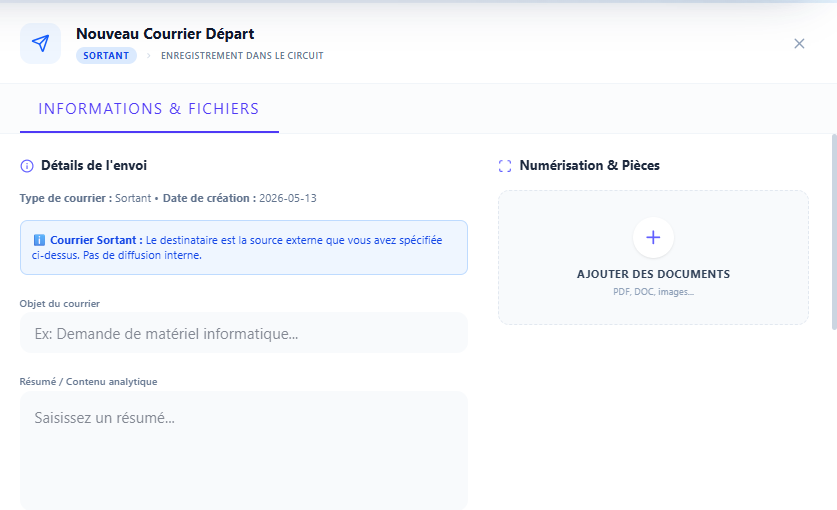
\includegraphics[width=\linewidth,height=0.36\textheight,keepaspectratio]{images/app/Courier_envoye_create.png}
    \end{minipage}
    \hfill
    \begin{minipage}{0.49\textwidth}
        \centering
        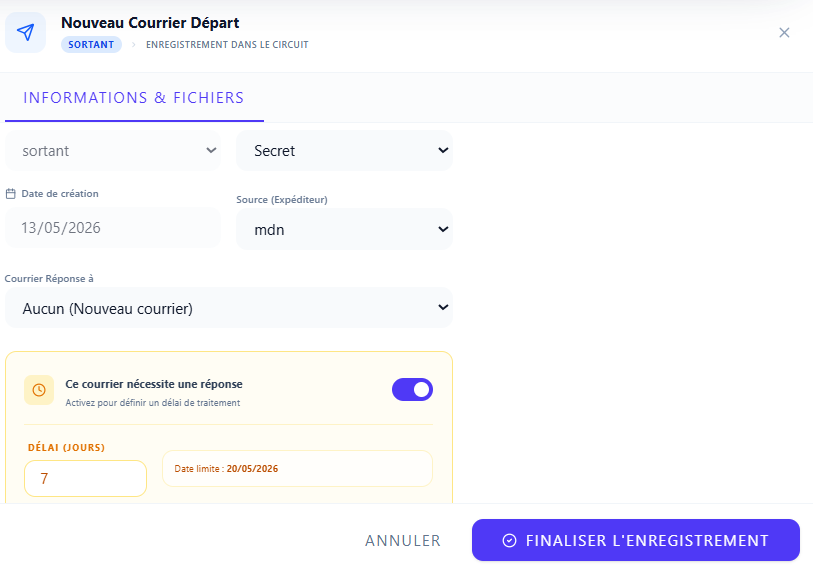
\includegraphics[width=\linewidth,height=0.36\textheight,keepaspectratio]{images/app/coureur_env_crea2.png}
    \end{minipage}
    \caption{Formulaire de création d’un courrier envoyé}
    \label{fig:creation_courrier_envoye}
\end{figure}

\subsection{Messagerie interne}
\label{subsec:messagerie_interne}

La messagerie interne sert à communiquer rapidement entre utilisateurs quand un courrier ne suffit pas. Elle permet d’envoyer et de recevoir des messages privés.

\begin{figure}[H]
    \centering
    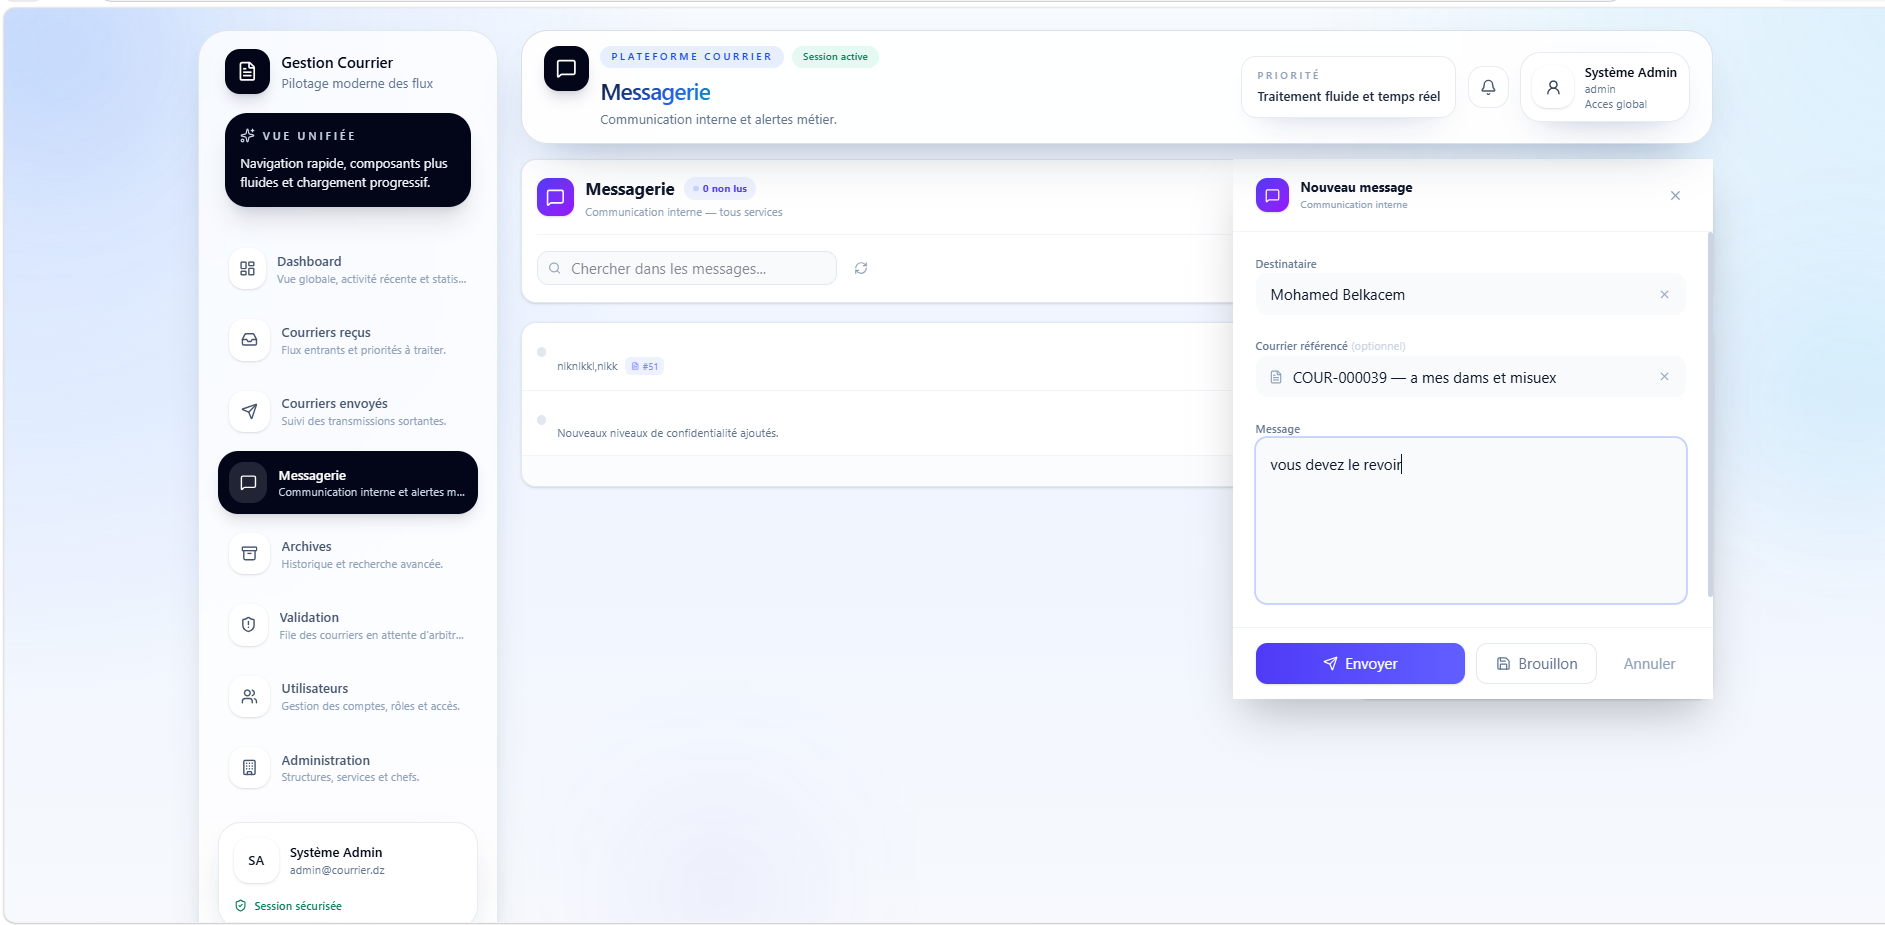
\includegraphics[width=0.90\textwidth,height=0.44\textheight,keepaspectratio]{images/app/msg_+create.png}
    \caption{Messagerie interne}
    \label{fig:messagerie_interne}
\end{figure}

\subsubsection{Création d’un nouveau message}
\label{subsubsec:creation_message}

L’utilisateur compose son message, choisit un destinataire et peut l’envoyer ou le sauvegarder en brouillon. C’est simple et direct.

\begin{figure}[H]
    \centering
    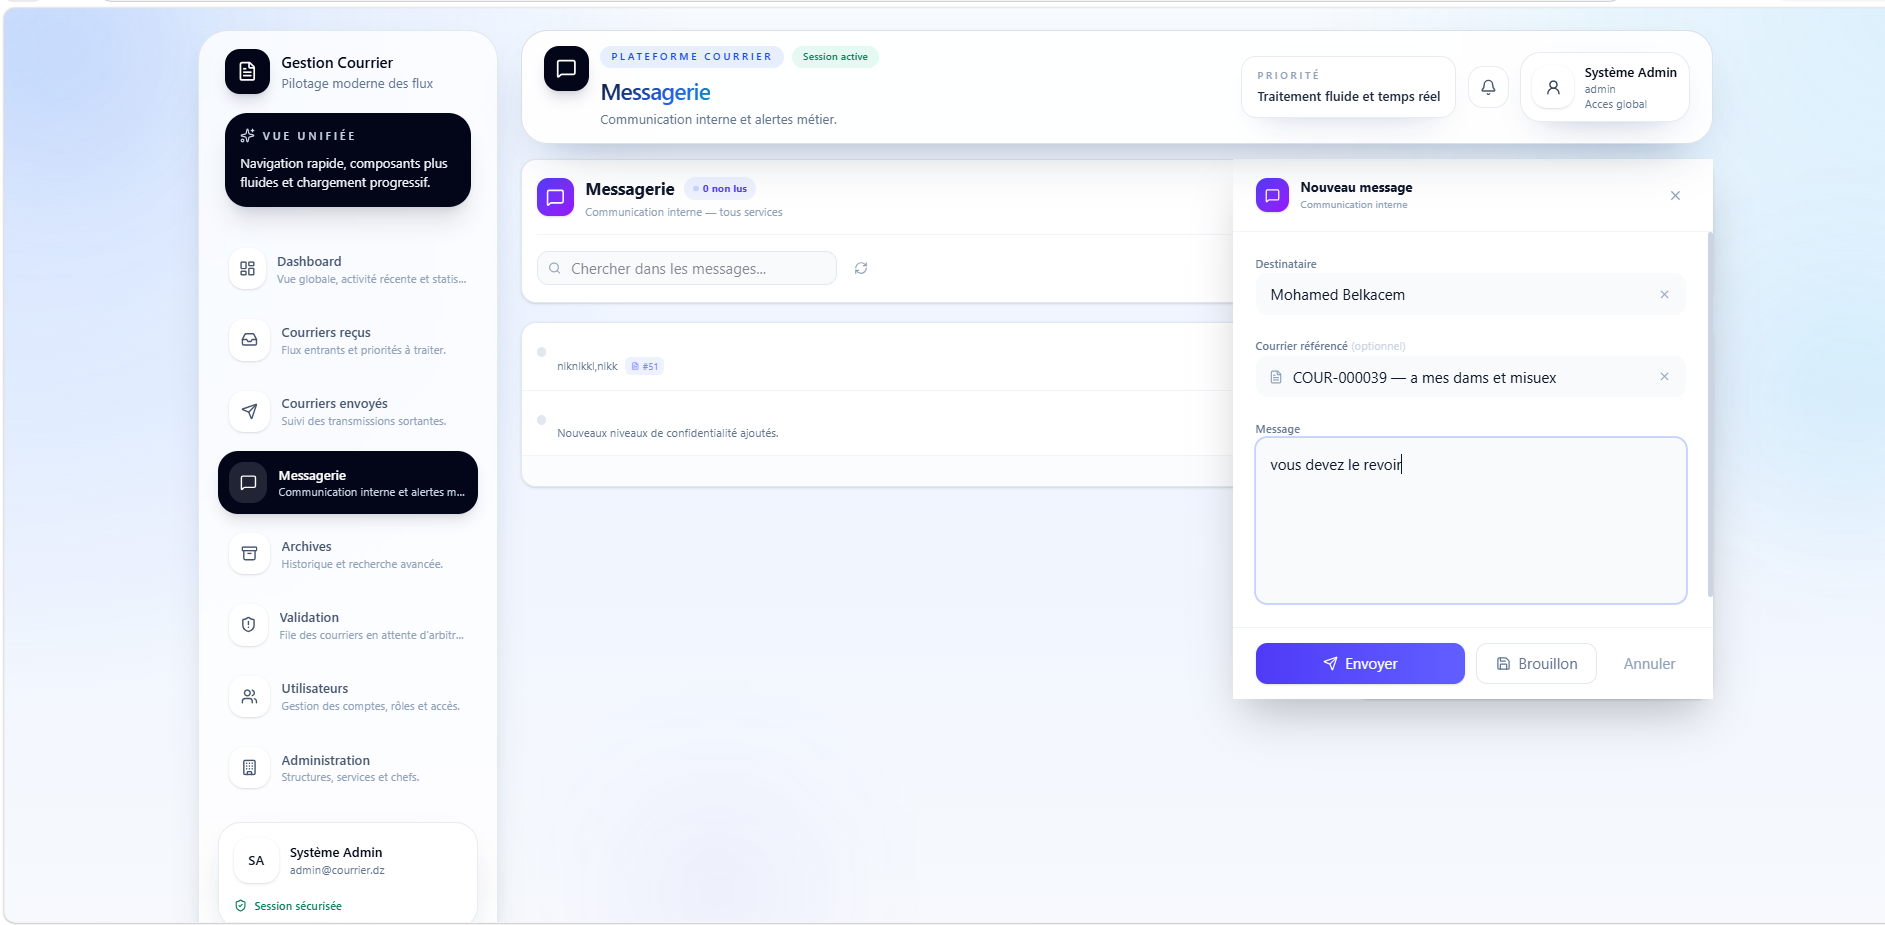
\includegraphics[width=0.90\textwidth,height=0.44\textheight,keepaspectratio]{images/app/msg_+create.png}
    \caption{Création d’un nouveau message}
    \label{fig:creation_message}
\end{figure}

\subsubsection{Consultation des messages}
\label{subsubsec:consultation_messages}

La consultation permet de lire les messages reçus et envoyés, avec le statut lu/non-lu et la possibilité de filtrer par destinataire.

\begin{figure}[H]
    \centering
    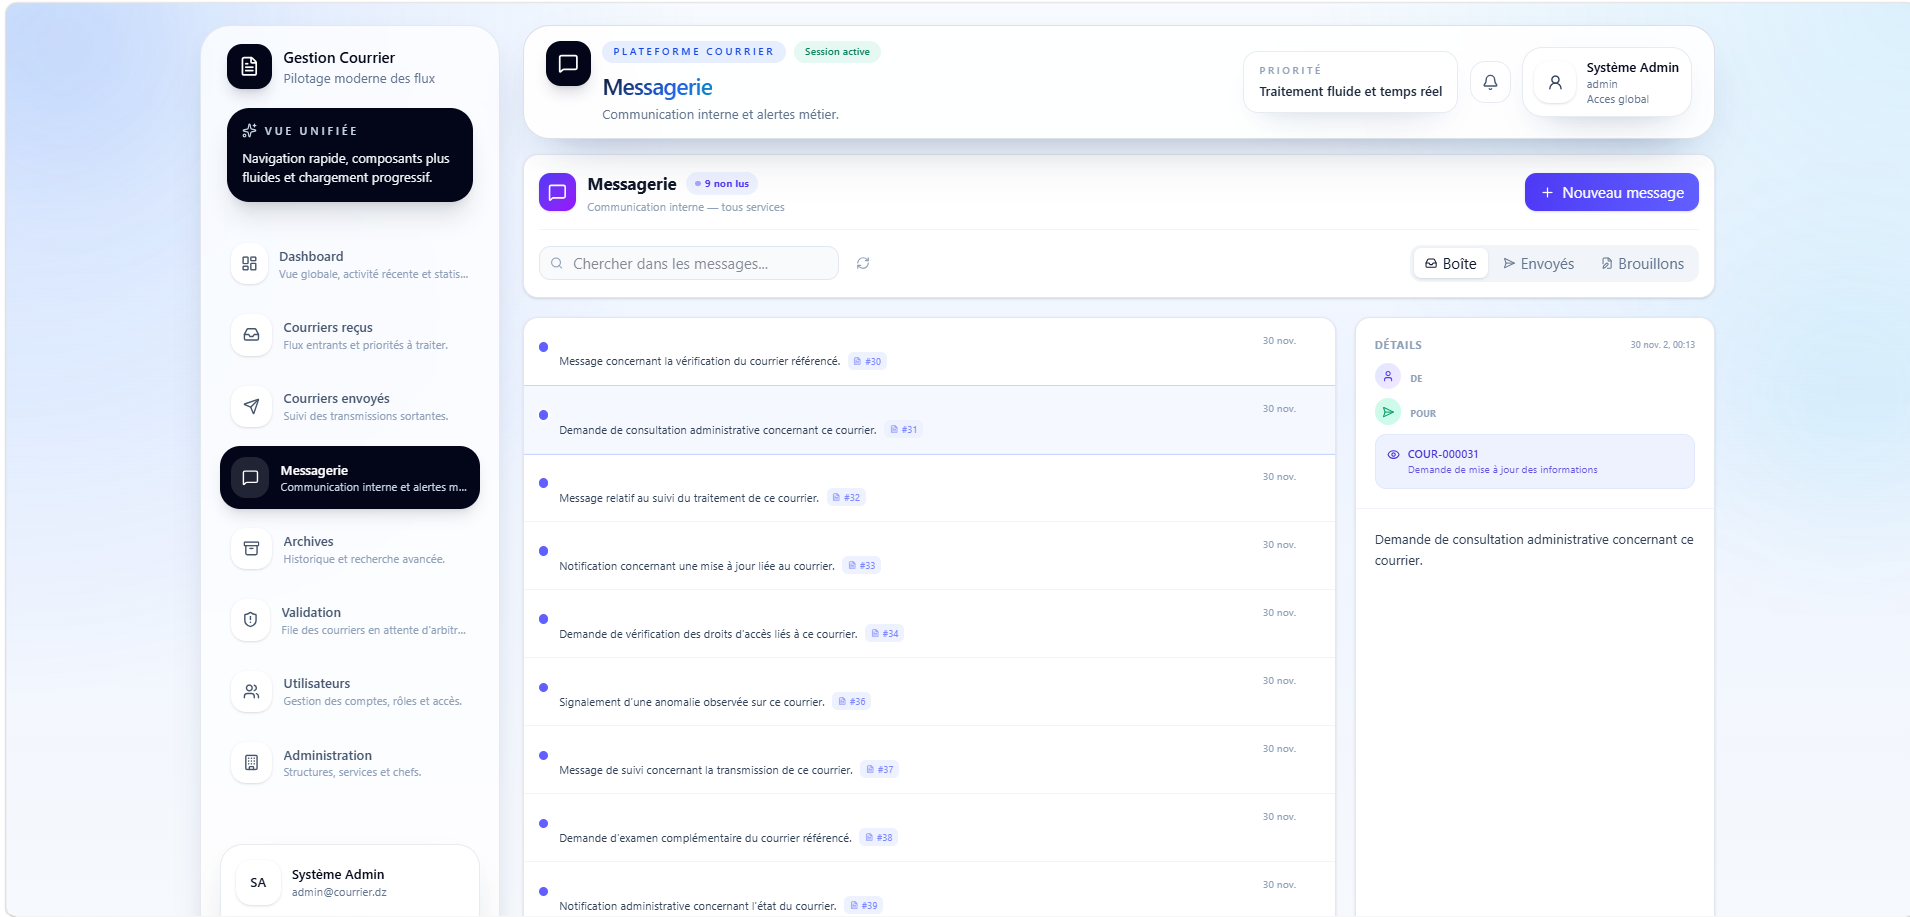
\includegraphics[width=0.90\textwidth,height=0.44\textheight,keepaspectratio]{images/app/cons_im.png}
    \caption{Consultation des messages}
    \label{fig:consultation_messages}
\end{figure}

\subsection{Gestion des archives}
\label{subsec:gestion_archives}

La gestion des archives permet de retrouver un courrier classé par le passé. C’est utile pour garder l’historique sans encombrer les listes actives.

\begin{figure}[H]
    \centering
    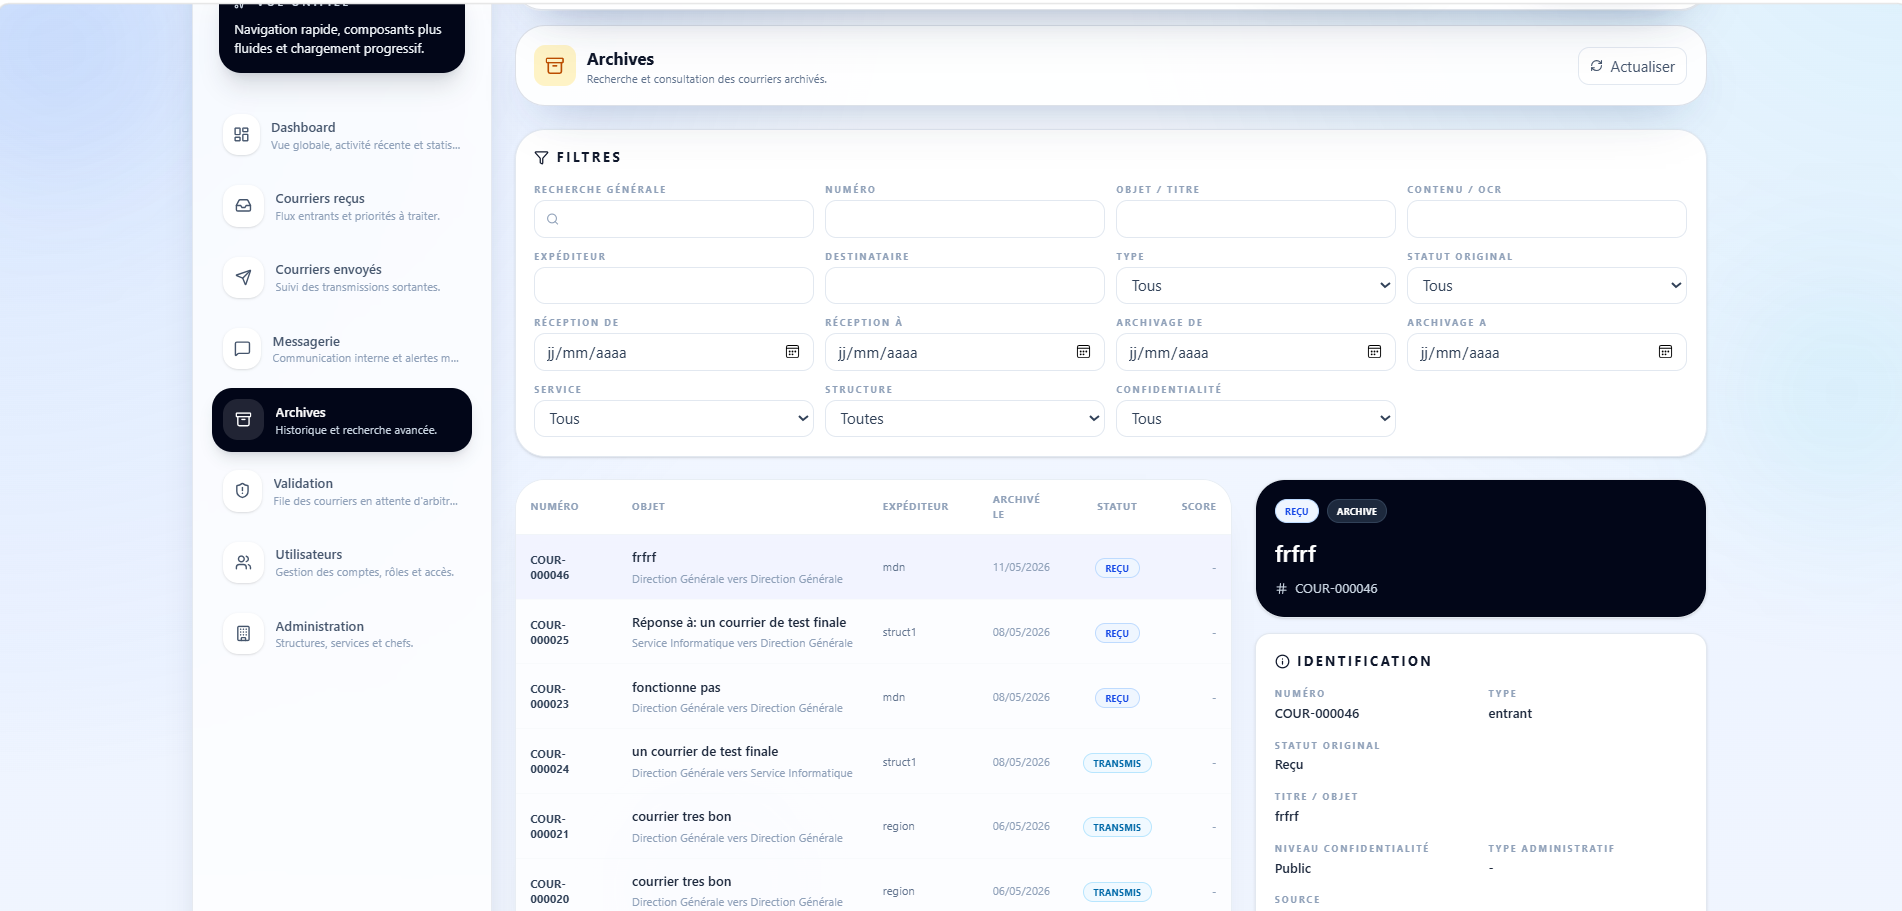
\includegraphics[width=0.90\textwidth,height=0.44\textheight,keepaspectratio]{images/app/archive.png}
    \caption{Vue de la gestion des archives}
    \label{fig:gestion_archives}
\end{figure}

\subsubsection{Recherche et filtrage des courriers archivés}
\label{subsubsec:recherche_filtre_archives}

Le moteur de recherche des archives accepte plusieurs critères : numéro, objet, date ou statut. Cela aide à retrouver rapidement un courrier ancien.

\begin{figure}[H]
    \centering
    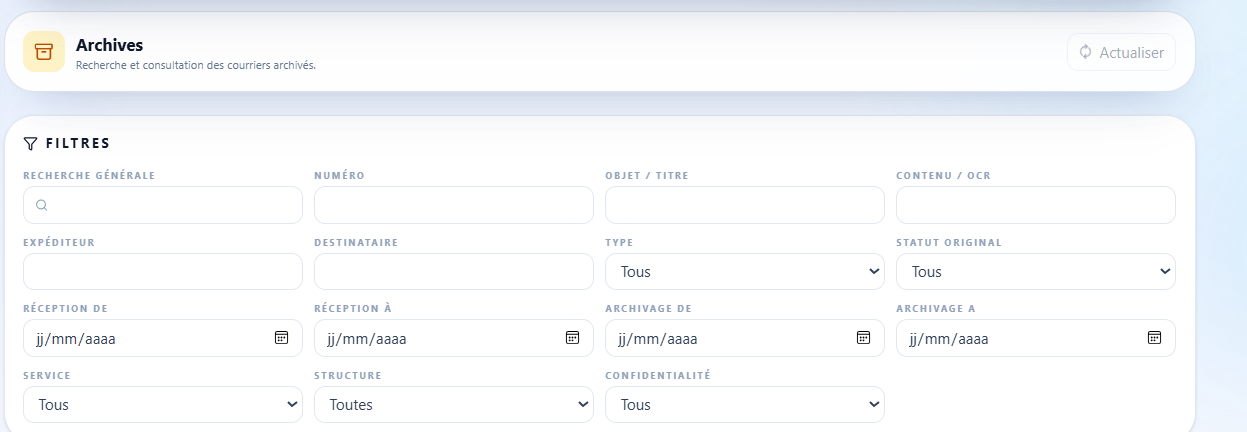
\includegraphics[width=0.90\textwidth,height=0.44\textheight,keepaspectratio]{images/app/filtre.png}
    \caption{Recherche et filtrage des archives}
    \label{fig:recherche_filtre_archives}
\end{figure}


\subsection{Gestion de l’administration}
\label{subsec:gestion_administration}

Cette partie est réservée à l’administrateur. Elle permet d’organiser les entités de l’application, notamment les structures, les services et l’affectation des responsables. Grâce à ces interfaces, l’administration peut préparer l’environnement de travail avant l’utilisation quotidienne du système par les autres profils.
\subsubsection{Gestion des utilisateurs}
\label{subsec:gestion_utilisateurs}

Cette page de gestion est destinée aux administrateurs. Elle affiche les profils utilisateurs, les rôles et les droits, et permet de modifier ou supprimer des comptes.

\begin{figure}[H]
    \centering
    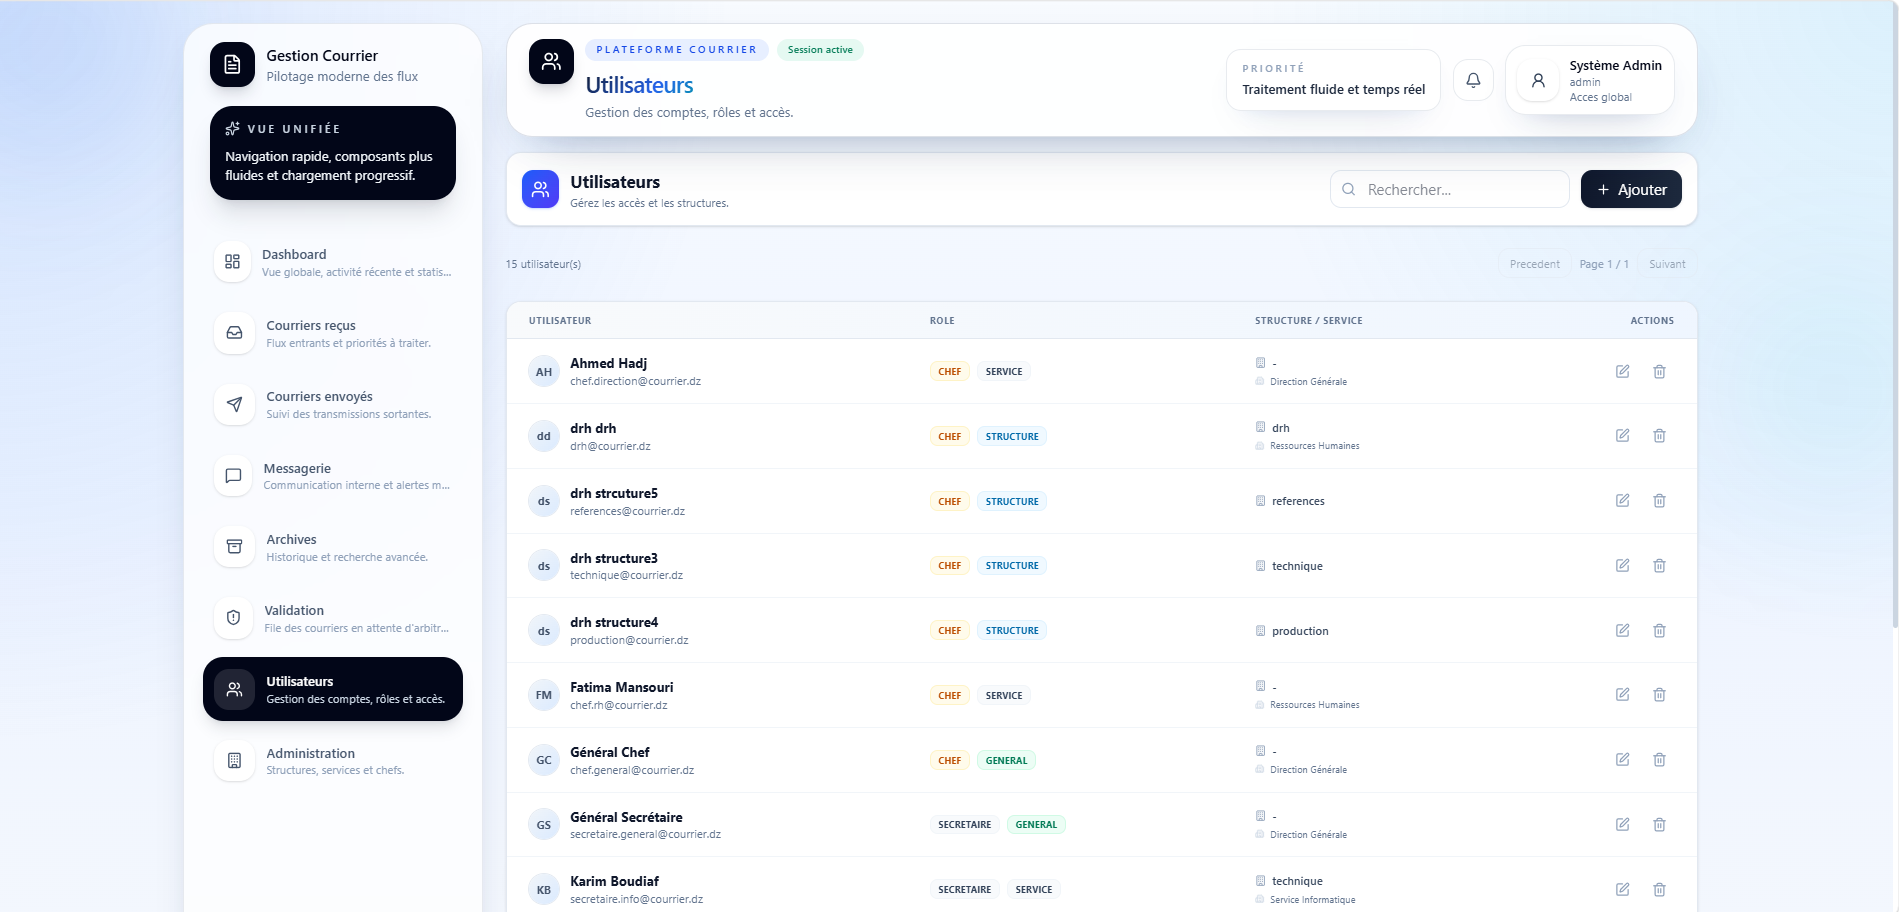
\includegraphics[width=0.90\textwidth,height=0.44\textheight,keepaspectratio]{images/app/users_index.png}
    \caption{Gestion des utilisateurs}
    \label{fig:gestion_utilisateurs}
\end{figure}

\subsubsection{Affichage des structures}
\label{subsubsec:affichage_structures}

L’affichage des structures permet à l’administrateur de consulter les différentes entités organisationnelles enregistrées dans l’application. Cette interface facilite le suivi des structures existantes et prépare les opérations d’ajout, de modification ou de suppression.

\begin{figure}[H]
    \centering
    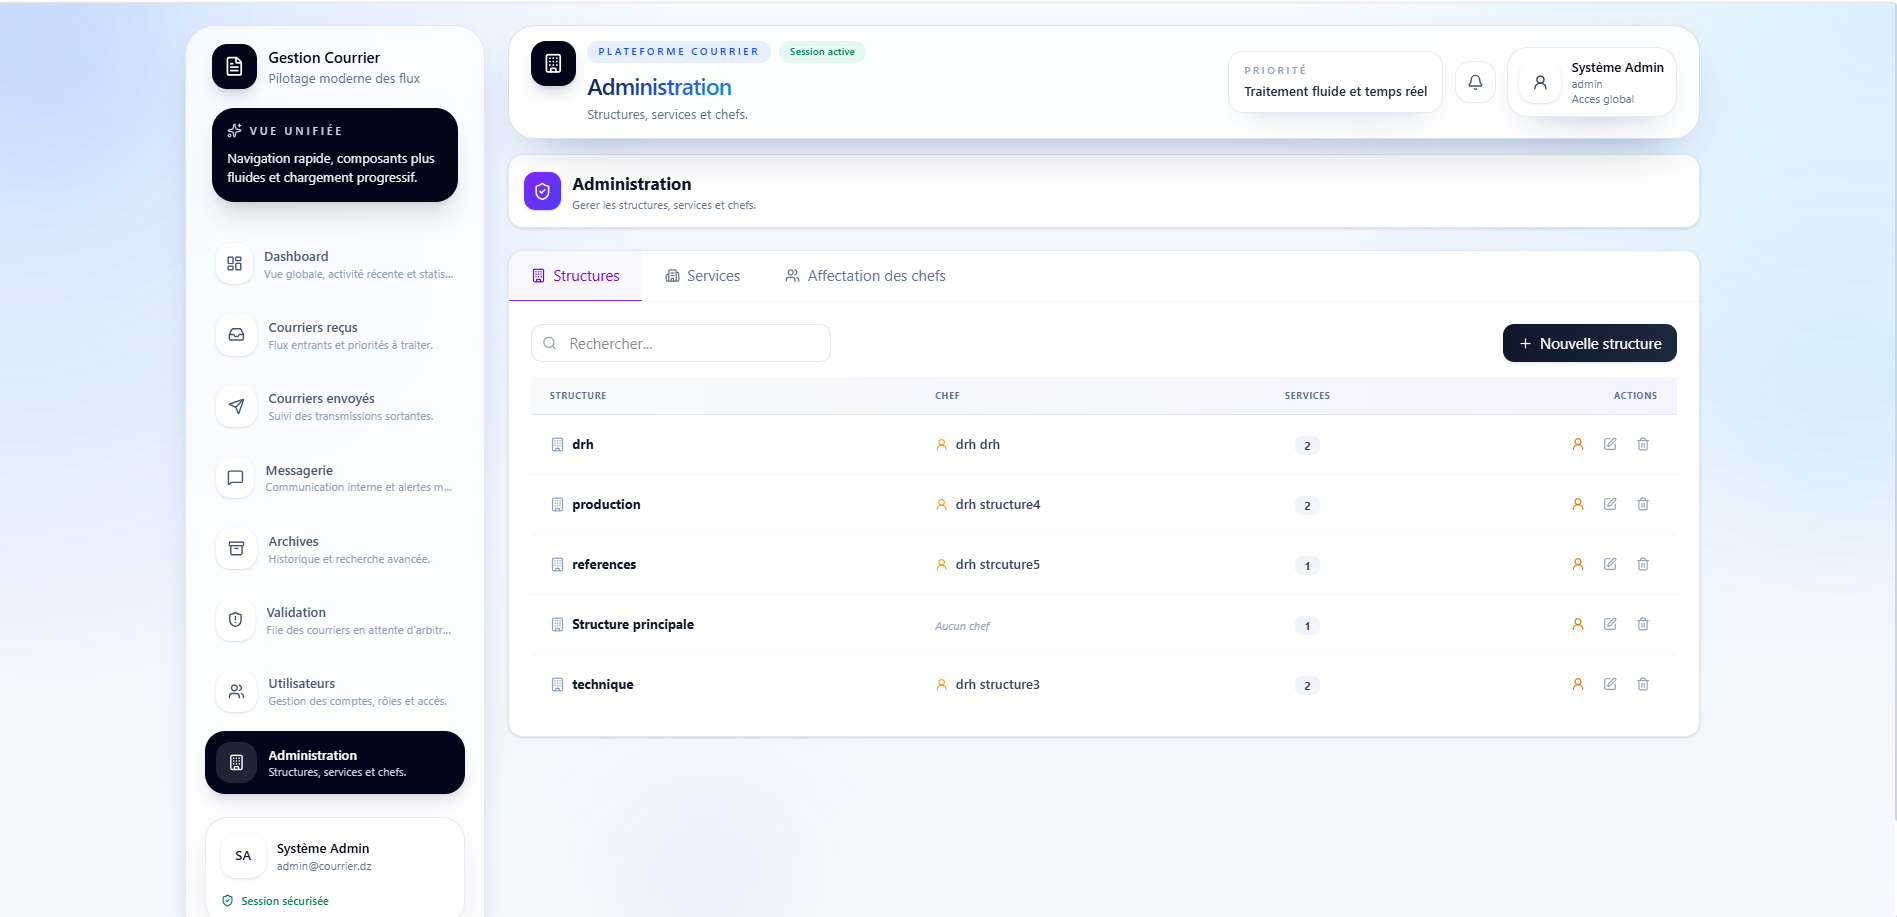
\includegraphics[width=0.92\textwidth,height=0.46\textheight,keepaspectratio]{images/app/adminstrationindex.png}
    \caption{Affichage des structures}
    \label{fig:affichage_structures}
\end{figure}

\subsubsection{Création d’une structure}
\label{subsubsec:creation_structure}

La création d’une structure permet d’ajouter une direction ou une entité organisationnelle dans le système. Cette structure pourra ensuite être utilisée pour rattacher des services et organiser les utilisateurs.

\begin{figure}[H]
    \centering
    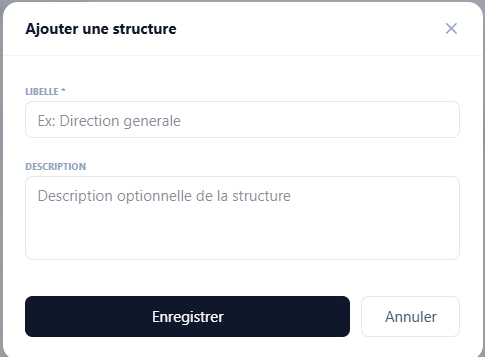
\includegraphics[width=0.88\textwidth,height=0.42\textheight,keepaspectratio]{images/app/struct_crr.png}
    \caption{Création d’une structure}
    \label{fig:creation_structure}
\end{figure}

\subsubsection{Affichage des services}
\label{subsubsec:affichage_services}

L’affichage des services présente la liste des services disponibles dans l’application. Chaque service est rattaché à une structure, ce qui permet de mieux organiser les utilisateurs et les circuits de traitement des courriers.

\begin{figure}[H]
    \centering
    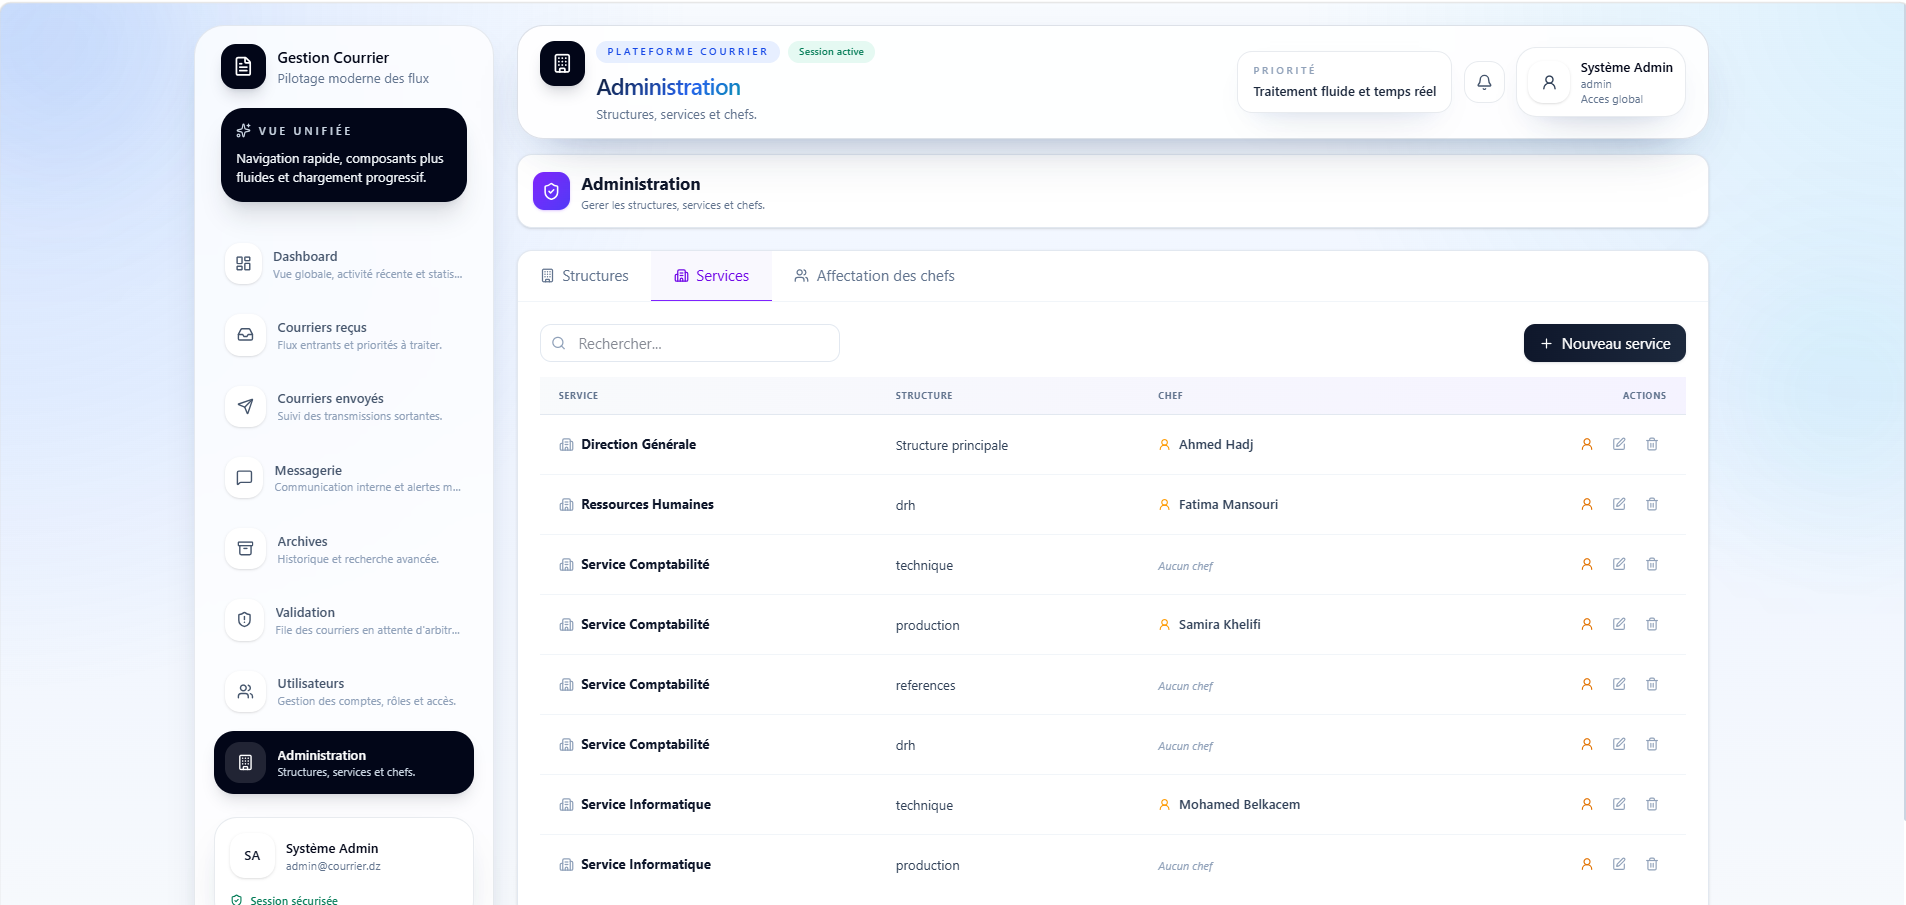
\includegraphics[width=0.92\textwidth,height=0.46\textheight,keepaspectratio]{images/app/services.png}
    \caption{Affichage des services}
    \label{fig:affichage_services}
\end{figure}

\subsubsection{Création d’un service}
\label{subsubsec:creation_service}

La création d’un service permet de définir les différents départements rattachés à une structure. Chaque service peut ensuite être utilisé dans la gestion des courriers, des utilisateurs et des droits d’accès.

\begin{figure}[H]
    \centering
    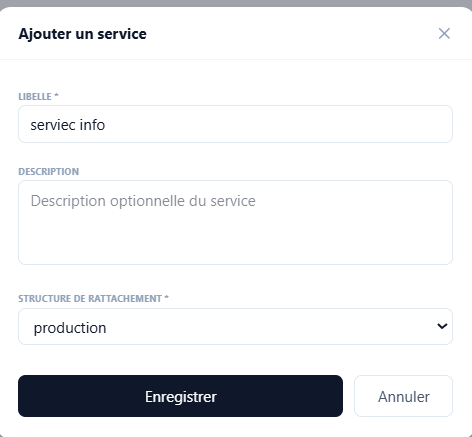
\includegraphics[width=0.88\textwidth,height=0.36\textheight,keepaspectratio]{images/app/services1.png}
    \caption{Création d’un service}
    \label{fig:creation_service}
\end{figure}

\subsubsection{Affectation des responsables}
\label{subsubsec:affectation_responsables}

L’affectation permet d’associer un responsable à une structure ou à un service. Cette étape est importante pour appliquer correctement les règles de validation, de transmission et de consultation des courriers selon le rôle de chaque utilisateur.

\begin{figure}[H]
    \centering
    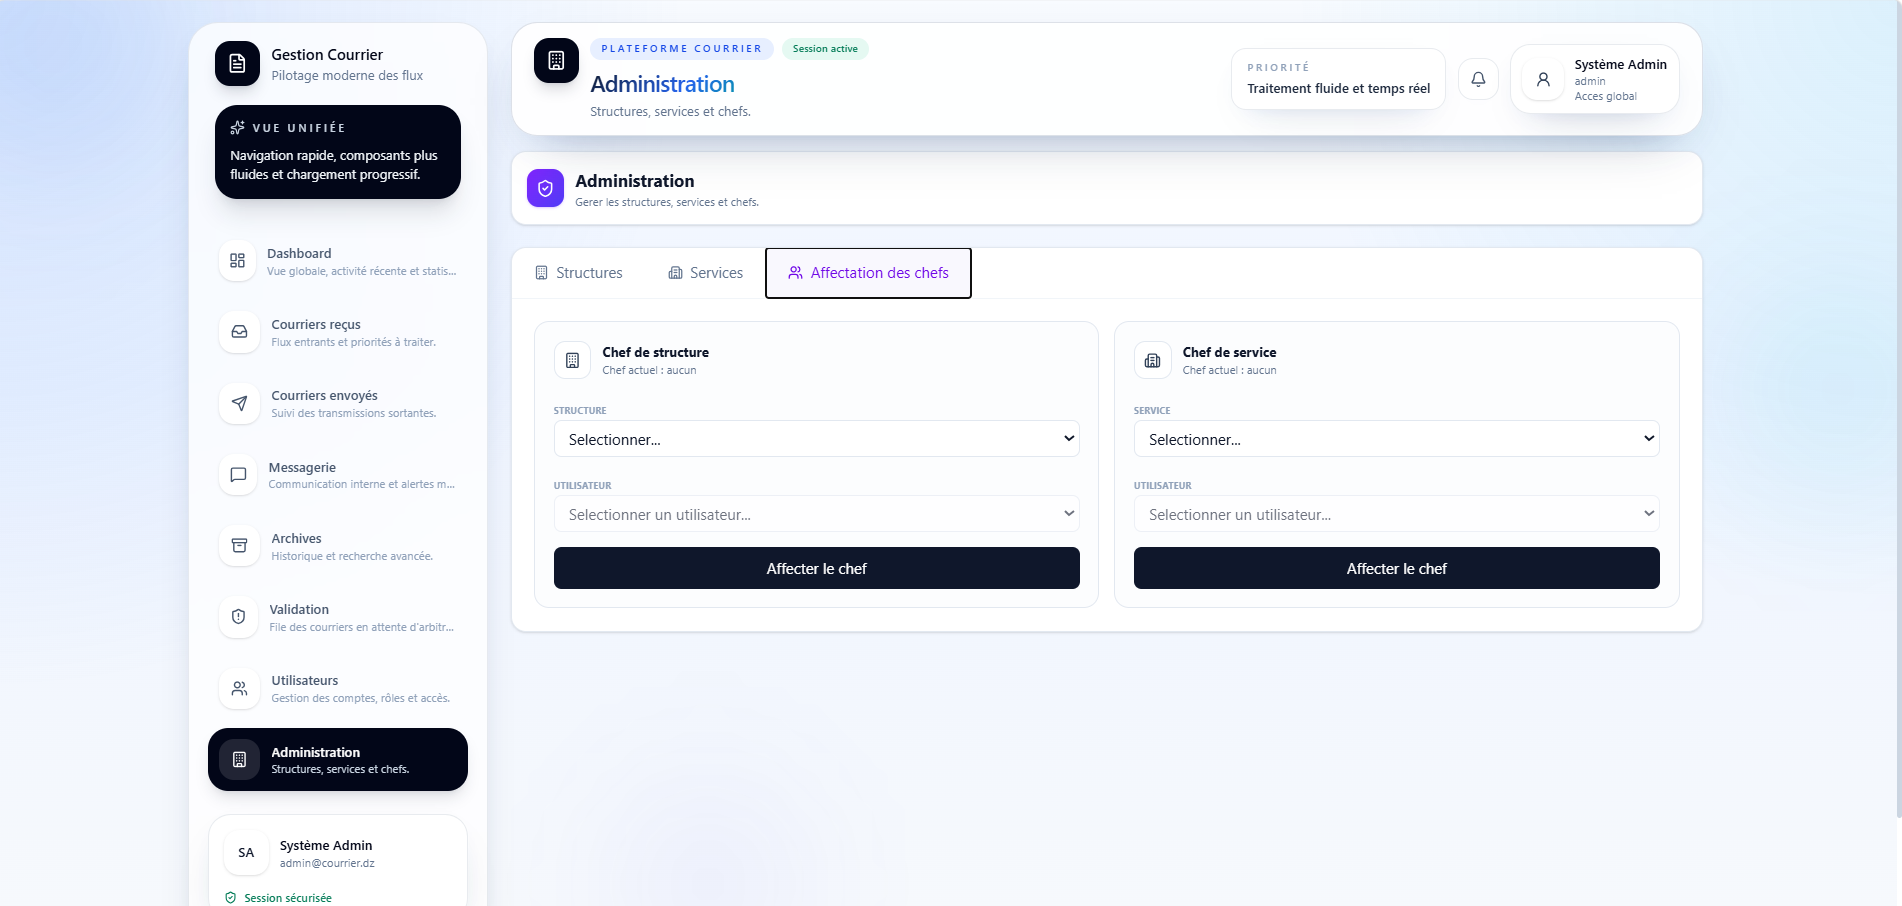
\includegraphics[width=0.88\textwidth,height=0.42\textheight,keepaspectratio]{images/app/affect.png}
    \caption{Affectation des responsables}
    \label{fig:affectation_responsables}
\end{figure}
\section{Conclusion}
\label{sec:conclusion_implementation}

Ce chapitre a présenté les principaux éléments liés à la réalisation de notre application web de gestion de courrier. Nous avons décrit les outils utilisés, l’architecture générale du système, le fonctionnement des échanges entre Laravel et React, ainsi que les principales interfaces développées. Cette étape permet de montrer comment les choix techniques ont été utilisés pour transformer la conception réalisée précédemment en une application fonctionnelle.
